\section{Integration}
\label{sec:integration}

\subsection{Structure of the generated code}

If during the code generation \emph{Compact code placement} was used, only four files are generated:

\begin{itemize}

    \item "system\_name".c
    \item "system\_name".h
    \item rtwtypes.h
    \item ert\_main.c

\end{itemize}

In the following we assume that the name of the Controller block was "controlsystem".

\begin{figure}[!ht]
    \centering
    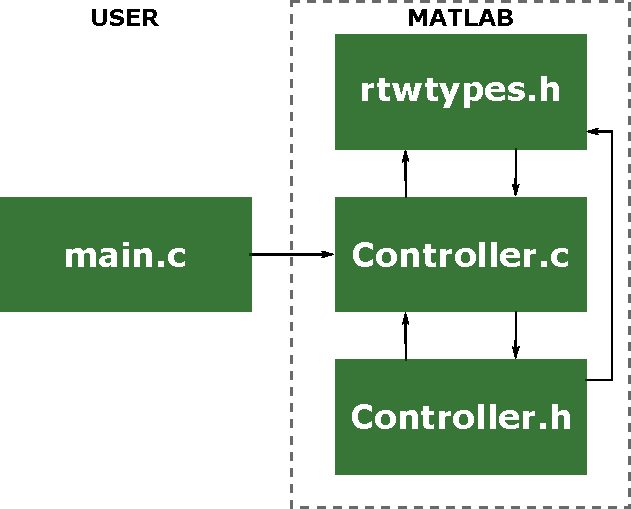
\includegraphics[width=0.6\linewidth]{img/rtw}
    \caption{Relationship of the generated files}
    \label{fig:rtw}
\end{figure}

The functions of the system are defined in the \textbf{controlsystem.c} and \textbf{controlsystem.h} files. The \textbf{rtwtypes.h} contains the unique type definitions of the code. The \textbf{ert\_main.c} is an exemplary main function that demonstrates the use of the others.

\subsection{Using the controller source code}

The generated source code is functionally a perfect equivalent of the \verb!Simulink! model. A number of functions and variable structures are defined that implement an easy interface of control the module, and communication with the system is only possible through this unique interface provided by the generated code. The system can be initialized using the \emph{controlsystem\_initialize()} function. It sets the 0 time in the model and the outputs obtain their initial values. The inputs are handled by the \emph{controlsystem\_U} struct. It contains fields each corresponding to a system input, matching it's name and type. If the inputs are set, calling the \emph{controlsystem\_step()} function runs the model once, for the period of one time sample. The outputs are stored in a structure similar to the input storage, called \emph{controlsystem\_Y}.

\subsection{Deployment with FreeRTOS on STM32F4-Discovery Board}

As in many controlled processes, the timing of the controller program execution is crucial, as well as processing the I/O lines, converting the analogue signals and sending status information to the supervisor computer over a wireless connection. It can be implemented with the integrated timer peripherals and interrupt sequences, but in case of a multi task system, the application of a \textbf{Real Time Operating System} allows a more high-level approach. There are numerous implementations of this operating system family. We chose FreeRTOS, a popular open-source operating system in the industry, because of its detailed documentation and earlier work experiences with the operating system on STM32F4-Discovery. In addition, it provides useful features for application debugging.

In our solution the FreeRTOS is responsible for the task scheduling, and provide a communication interface between the tasks. This way we can ensure that the sensor readings and the controller task are conducted with precise timing. Through the operating system direct communication with the I/O lines are simple, and it handles the reading of the optoelectronic and proximity sensors and their processing on the Analogue to Digital converters of the board.
%Freertos mint Core mit csinál? (beszélget a hardverrel, szenzorokkal, aktuárotoknak küld beavatkozó jeleket)
%Miért jó? (gyors hozzáférés a szenzorokhoz, pontos ütemezés a controllernek)

Setting up the system is quite easy in this point. We only have to include the FreeRTOS source files into our project.\footnote{A detailed description is available for many processors in the FreeRTOS website: http://www.freertos.org/} The next step is to write some low level driver to read the sensors, and initialize the actuators so this way we can connect these to the control system. It is also necessary to set up the communication between the tasks, so we can read the state of the controller and the other tasks real time.
%Mit kellett csinálni, hogy működjön? (FreeRTOS-t feltenni rá (max 1 mondat, ebbe nem megyünk bele!), hardver jeleket kiolvasni C-vel, hogy oda tudjuk adni a controllernek, matlab-ot rákötni egy interrupt-ra)
%Még mit kell csinálni, hogy működjön?? Max 1-2 mondat már csak.